% Proposed definition of the SPIF raw instrument data format
\documentclass[12pt,a4paper]{article}
%\usepackage[none]{FAAM_StdDoc}
\usepackage[T1]{fontenc}
\usepackage{helvet,mathptmx,graphics}
\usepackage[pdftex,colorlinks=true]{hyperref}
\usepackage{ifthen,calc}
\usepackage[usenames,dvipsnames]{color}
\usepackage{fancyhdr}
\usepackage{graphics}
\usepackage{booktabs,longtable}

% Set longtable margins to textwidth
\setlength\LTleft{0pt}
\setlength\LTright{0pt}
\setlength{\LTcapwidth}{\textwidth}

% Limit the depth of the table of contents to subsections
%\setcounter{tocdepth}{2}

% Set manually fixed text width
\newlength{\texttablecolwidth}
\setlength{\texttablecolwidth}{11cm}


% Define list for variables for netCDF files
\newcommand{\varlabel}[4][None]%
    {\footnotesize\textit{#2}~\texttt{#3}#4\ifthenelse{\equal{#1}{None}}%
                                           {\rule{0pt}{1ex}}%
                                           {~=~#1;}\normalsize}

% Define a max width of varitem. If varitem is greater than varitemwidth
% then put item text on next line.
\newlength{\varitemwidth}
\setlength{\varitemwidth}{3.5cm}
\newlength{\vartextwidth}
\setlength{\vartextwidth}{0.5\textwidth}

\newlength{\Mylen}
\newcommand{\varlistlabel}[1]%
    {\settowidth{\Mylen}{#1}%
     \ifthenelse{\lengthtest{\Mylen>\labelwidth}}%
                % if label > labelwidth
                {\parbox[b]{\labelwidth}% 
                {\makebox[0pt][l]{#1}
                 \mbox{}\\}}%
                % else if label < labelwidth
                {#1}%
     \hfil\relax}

\newenvironment{varlist}[4][None]%
% Three args are value [none], type, name, (dim)
% (dim) is a bit of a cludge. If none then give {}
    {\vspace{1ex}
     \noindent
     \varlabel[#1]{#2}{#3}{#4}
     \begin{list}{}{%
        \footnotesize%
        \renewcommand{\makelabel}[1]{\varlistlabel{\quad \texttt{#3:##1}~=}}%
        % Vertical seperations
        \setlength{\parsep}{0ex}%
        \setlength{\partopsep}{0.25ex}%
        \setlength{\topsep}{0.25ex}%
        \setlength{\itemsep}{0.25ex}%
        % Horizontal seperations
        \setlength{\itemindent}{0cm}%
        \setlength{\listparindent}{0cm}%
        \setlength{\labelwidth}{\varitemwidth}%
        \setlength{\labelsep}{0em}%
        \setlength{\leftmargin}{\labelwidth+\labelsep}%
        \setlength{\rightmargin}{0cm}}}%
    {\normalsize\end{list}}



\begin{document}

\title{SPIF--Single Particle Image Format}
\author{The SPIF Working Group}
%\docver{0.1}
%\docnum{}
\date{November 2016}
%\docURL{Link to webpage when written}
%\docrelated{FAAM000002}

\maketitle
\begin{abstract}
This document defines the Single Particle Image Format (SPIF) file structure and and variables. The SPIF file is a HDF5 file and a universal file format for single particle image probe data.
\end{abstract}
\tableofcontents
%\pagebreak


\section{Motivation}
A variety of file formats are used by particle imaging instrument manufacturers. The formats are dictated by hardware and bandwidth limitations, and so may not have a convenient or conventional structure. However, after data has been acquired, and as hardware improves, the imposed limitations vanish. We propose a new file format for these imaging probes. The new format will specify a single structure which all imaging probe data formats may be mapped onto, leading to improved accessibility for users and refinement of data processing routines. We aim for this format to be adopted by instrument manufacturers. The format is also suitable for representing historical datasets and is suitable for long term archiving of raw data. File converters for some of the most commonly used probes are provided.


\section{Description}
The SPIF file format uses the HDF5 format. HDF5 is a structured binary file format capable of containing large datasets and has automatic compression utilities. HDF5 is widely supported on a variety of platforms and environments. 
\par
Datasets will be contained in groups within a SPIF file. Only data from a single instrument may be stored in a given group although SPIF files can contain data from multiple instruments through the use of multiple groups.
Metadata will be provided for each instrument to provide information on data sources etc.

\section{SPIF File Definition}
\label{sec:FileDefinition}

\begin{description}
\item[root] The root of the file contains global attributes.
\item[instrument group] Each instrument data included within the file has a seperate group.
\begin{description}
\item[root] Instrument metadata
\item[core] The SPIF-Core group contains the data necessary for subsequent analysis
\item[aux] The SPIF-Aux group contains additional data which is generated by a given instrument, but is not essential for data processing. This data is included to maintain integrity of the original dataset, making SPIF a suitable format for long term archiving.
\item[lvlX] Processed data may be included as a subgroup of either \texttt{core} or \texttt{aux} or as individual variables within the same group but with an appropriate \texttt{level} attribute.
\end{description}
\end{description}

\subsection{SPIF root}

The root of the SPIF file has all of the global data and attributes relating to the production of the file.
\\[2em]
\varlabel[``SPIF--Single Particle Image Format'']{char}{title}{}\marginpar{\scriptsize$\leftarrow$I'm actually not keen on this name, though the acronym is cool, as it limits the scope of the format.}\\
\varlabel[Institution that produced the file]{char}{institution}{}\\
\varlabel[Version of processing code]{char}{source}{}\\
\varlabel[Link to web, paper, document reference describing datasets, project, etc]{char}{references}{}\\
\varlabel[creation/modification datetime, version number]{char}{history}{}\\
\varlabel[datetime, comment, changelog(?)]{char}{comment}{}\\
\\
\varlabel[Name of project]{char}{project}{}\\
\varlabel[Reference date of all datasets]{char}{start\_date}{}
\marginpar{\scriptsize$\leftarrow$Will all the datasets have a common start date and project? If notmove these to instrumet group roots.}\\

\subsection{Instrument group}

The root of the instrument group contains information pertaining to the individual instrument. It may also include information about the probe software module that was used to create it, this may be different to the version of the overal processing code.
\\[2em]
\varlabel[Full descriptive name of instrument (name of group is instrument standard name]{char}{instrument\_long\_name}{}\\
\varlabel[Institution operating instrument]{char}{institution}{}\\
\varlabel[Link to web, paper, document reference describing instrument]{char}{reference}{}\\
\varlabel[Serial number or instrument identifier]{char}{instrument\_serial\_number}{}\\
\varlabel[Manufacturer of instrument]{char}{manufacturer}{}\\
\\
\varlabel[Instrument firmware version]{char}{instrument\_firmware}{}\\
\varlabel[Instrument software version]{char}{instrument\_software}{}\\
\varlabel[Name or description of platform instrument is mounted on]{char}{platform}{}\\
\varlabel[Any further notes about instrument, platform, location, orientation, etc]{char}{comment}{}\\
\par
Although envisaged to be used exclusively with optical array probes, there is no reason that this format could not be used for any instrument type. Therefore there may not be suitable universal descriptive attributes for all instrument types. It may thus be desirable that these attributes are placed in a sub-group although this may add a layer of complexity for little gain. Below are variables which may be used for an optical array probe.

\begin{varlist}{int}{pixels}{(len of array)}
\item[long\_name] Vector of pixel numbers for \texttt{instrument};
\item[comment] Any relevant comments;
\end{varlist}

\begin{varlist}{float64}{resolution}{(scalar or 2)}
\item[long\_name] Physical resolution of array pixels \texttt{instrument};
\item[units] ``micrometer'';
\item[ancillary\_variables] \texttt{instrument:resolution\_err};
\item[comment] Any relevant comments;
\end{varlist}

\begin{varlist}{float64}{resolution\_err}{(scalar or 2)}
\item[long\_name] Uncertainty of physical resolution of array pixels \texttt{instrument};
\item[units] \texttt{instrument:resolution};
\item[comment] Any relevant comments;
\end{varlist}

\begin{varlist}{float64}{arm\_seperation}{}
\item[long\_name] Physical distance between probe arms;
\item[units] ``millimeter'';
\item[ancillary\_variables] \texttt{instrument:arm\_seperation\_err};
\item[comment] Any relevant comments;
\end{varlist}

\begin{varlist}{float64}{arm\_seperation\_err}{}
\item[long\_name] Uncertainty of physical distance between probe arms;
\item[units] \texttt{instrument:arm\_seperation};
\item[comment] Any relevant comments;
\end{varlist}

\begin{varlist}{boolean}{antishatter\_tips}{}
\item[long\_name] ``Use of antishatter-, or Korolev-, tips on probe arms.'';
\item[comment] Any relevant comments;
\end{varlist}

\begin{varlist}{int}{bpp}{}
\item[long\_name] ``Bits per pixel used in image data'';
\item[comment] Any relevant comments;
\end{varlist}

\begin{varlist}{int}{channels}{}
\item[long\_name] ``Number of measurement channels of instrument'';
\item[comment] Any relevant comments;
\end{varlist}


\subsection{Instrument Core}

The Instrument Core group contains data necessary for analysis and processing of the raw data. There is a single coordinate for all variables in this group. This does mean that some of the arrays are larger than would otherwise be the case but it does mean that all the arrays are the same length which makes for more efficient storage and chunking. The coordinate is time, the length of \texttt{particle\_ns} defines the length of the coordinate dimension, where the arrival time of the $n$th particle is given by \texttt{particle\_ns}($n$) + \texttt{particle\_sec}($n$).
\par
Some probes will have multiple channels, for example the 2DS has two orthogonal arms. Using a single coordinate for the group means that the time stamps of the two channels must be the same.\marginpar{\scriptsize$\leftarrow$Is this the case for these probes?} This will be fine for instruments with different polarisation-sensitive channels as well. Thus for a probe that is made up of multiple instruments, for example the 3V-CPI, where the particle detection will not be coincident, data will have to be split into different instrument groups.
\par
There are several ways to hold data from multiple channels. One is to increase the depth of the data array to accommodate each additional channel. The other is to increase the number of variables. The former has the advantage of a consistant number of variable names in the group, the latter the advantage of simpler array structures which may be more convenient for probe data that is already complicated. The variables described here assume the former structure.
\par
The instrument core data group consists of:

\begin{varlist}{float}{particle\_ns}{(time)}
\item[standard\_name] ``time'';
\item[long\_name] ``particle arrival time in nanoseconds'';
\item[units] ns since \texttt{particle\_sec};
\item[ancillary\_variables] \texttt{particle\_sec};
\item[comment] Any relevant comments;
\end{varlist}

\begin{varlist}{int}{particle\_sec}{(time)}
\item[long\_name] ``particle arrival time in seconds'';
\item[timezone] ``UTC'';
\item[units] ``seconds since \texttt{start\_date} 00:00:00'';
\item[strftime\_format] ``\%F \%T \%Z'';
\item[comment] Any relevant comments;
\end{varlist}

\begin{varlist}{int}{particle\_image}{(time,pixels,channels)}
\item[long\_name] ``Particle image array'';
\item[ancillary\_variables] 
\item[\_FillValue] -9999.f (?);
\item[comment] Any relevant comments;
\end{varlist}

\begin{varlist}{boolean}{overload}{(time,channels)}\marginpar{\scriptsize$\leftarrow$Is this going to be per channel or for all channels?}
\item[long\_name] ``Probe particle overload status'';
\item[comment] Any relevant comments;
\end{varlist}

\textbf{I'm not sure what this refers to:}\\
Indexes to relate any given particle event/time stamp to the corresponding data stored in the image array


\subsection{Instrument Aux}

The Instrument Aux group contains auxillary data which is generated by a given instrument, but is not essential for data processing. This data is included to maintain integrity of the original dataset, making SPIF a suitable format for long term archiving. This group has its own time coordinate, this accommodates 1~Hz one dimensional data that may be transmitted in parallel to the two dimensional image data.

\begin{varlist}{int}{time}{(time)}
\item[standard\_name] ``time'';
\item[long\_name] ``time in seconds'';
\item[timezone] ``UTC'';
\item[units] ``seconds since \texttt{start\_date} 00:00:00'';
\item[strftime\_format] ``\%F \%T \%Z'';
\item[comment] Any relevant comments;
\end{varlist}

Variables in this group will be instrument-specific but may include:
\begin{itemize}
\item Housekeeping data
\item Buffer time stamps
\item Particle counters
\item Data acquisition timing words.
\item Probe airspeed data
\end{itemize}


\subsection{Level \textit{n} processed data}

It may be desirable to include some processed data along with the unadulterated raw particle data. These variables should include an \texttt{level} attribute to indicate the appropriate processing level applied;
\begin{description}
\item[level 0] Raw, or pixel, units\marginpar{\scriptsize$\leftarrow$Should all unadulterated raw data, eg \texttt{particle\_image} include a \texttt{level} of 00?}
\item[level 1] Geophysical units
\item[level 2] Bulk properties in geophysical units?
\end{description}
\par
The variables could be included in a subgroup of the Instrument core or aux groups. Where it is placed will depend on the appropriate coordinate time. For example, level 0 data could be placed within the core group as these variables will use the same nanosecond and seconds time coordinates as the raw single particle data. Level 2 data such as total concentration and median volume diameter will use the same time coordinates as probe air speed data so would probably be put in a subgroup of the aux group.
\par
For monoscale image probes level zero processed data may include;
\begin{itemize}
\item Single particle properties 
\item Area
\item Filled Area
\item Perimeter
\item Position on Array
\item Num Edge0 Pixels On
\item Num Edge1 Pixels On
\item Dmax, Dx, Dy etc etc
\item Number of particles in image event
\item Corrections to dead pixels?
\end{itemize}


\section{SPIF Code Definitions}

Code that produces the SPIF files is written in python~3 using the h5py module to interface with the hdf5 library. The structural layout of the code is shown in figure~\ref{fig:SoftwareStructure}.
\begin{figure}
\begin{center}
\resizebox{0.5\linewidth}{!}{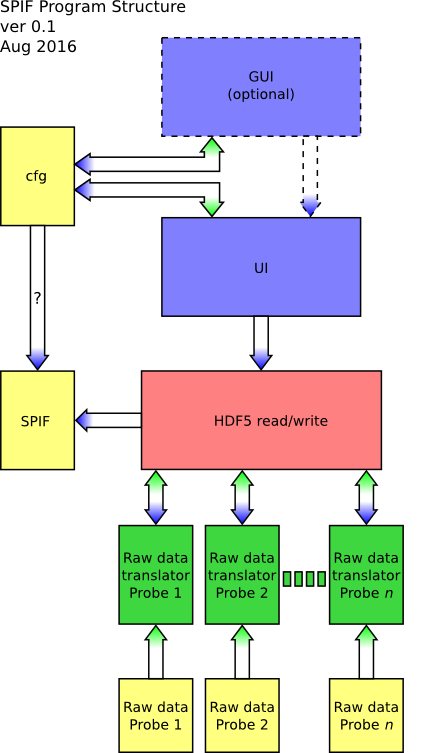
\includegraphics{images/SPIF_program_structure}}
\caption{Functional diagram of possible software structure. Using self-contained layers and algorithm functions should more easily allow code additions and modification. See text for more details.\label{fig:SoftwareStructure}}
\end{center}
\end{figure}
The code is organised in different layers, the lowest level being the raw data translator shown in figure~\ref{fig:SoftwareStructure} in green. These code functions read in the raw data from the probe and put it into variables that are easily digested by the hdf5 read/write layer, down in pink.
\par
The h5py module accepts python dictionaries and numpy variables and iterables. Eventually this section will describe the details of the expected outputs of the data translators however at this stage it should be reasonably obvious from the hdf5 structures given in section~\ref{sec:FileDefinition}. Each hdf5 group will be a dictionary, with each variable being a subdictionary with the attributes of these variables being either native python or numpy variables types.

\subsection{Data Chunking}

It is quite possible for a translator to read in an entire raw data file for a single probe, parse that into the appropriate (and possibly large) python variables, and pass the resultant dictionary to the hdf5 read/writer module for writing into the SPIF file. This would result in on-the-fly chunking and filtering by the hdf5 library. It is also possible that the raw data files are too numerous or large to be handled all together and so subsets of the data need to be streamed to the read/write module piecemeal. This will also occur if the SPIF file is being written in realtime. This will mean that chunking and filtering may have to be set manually. Thus there may be information passed from the translator to the read/write module that is not stored in the SPIF file but is used to construct the SPIF file.






\label{LastPage}
\end{document}
